\documentclass{standalone}
\usepackage{tikz}
\usetikzlibrary{patterns, positioning}


\begin{document}
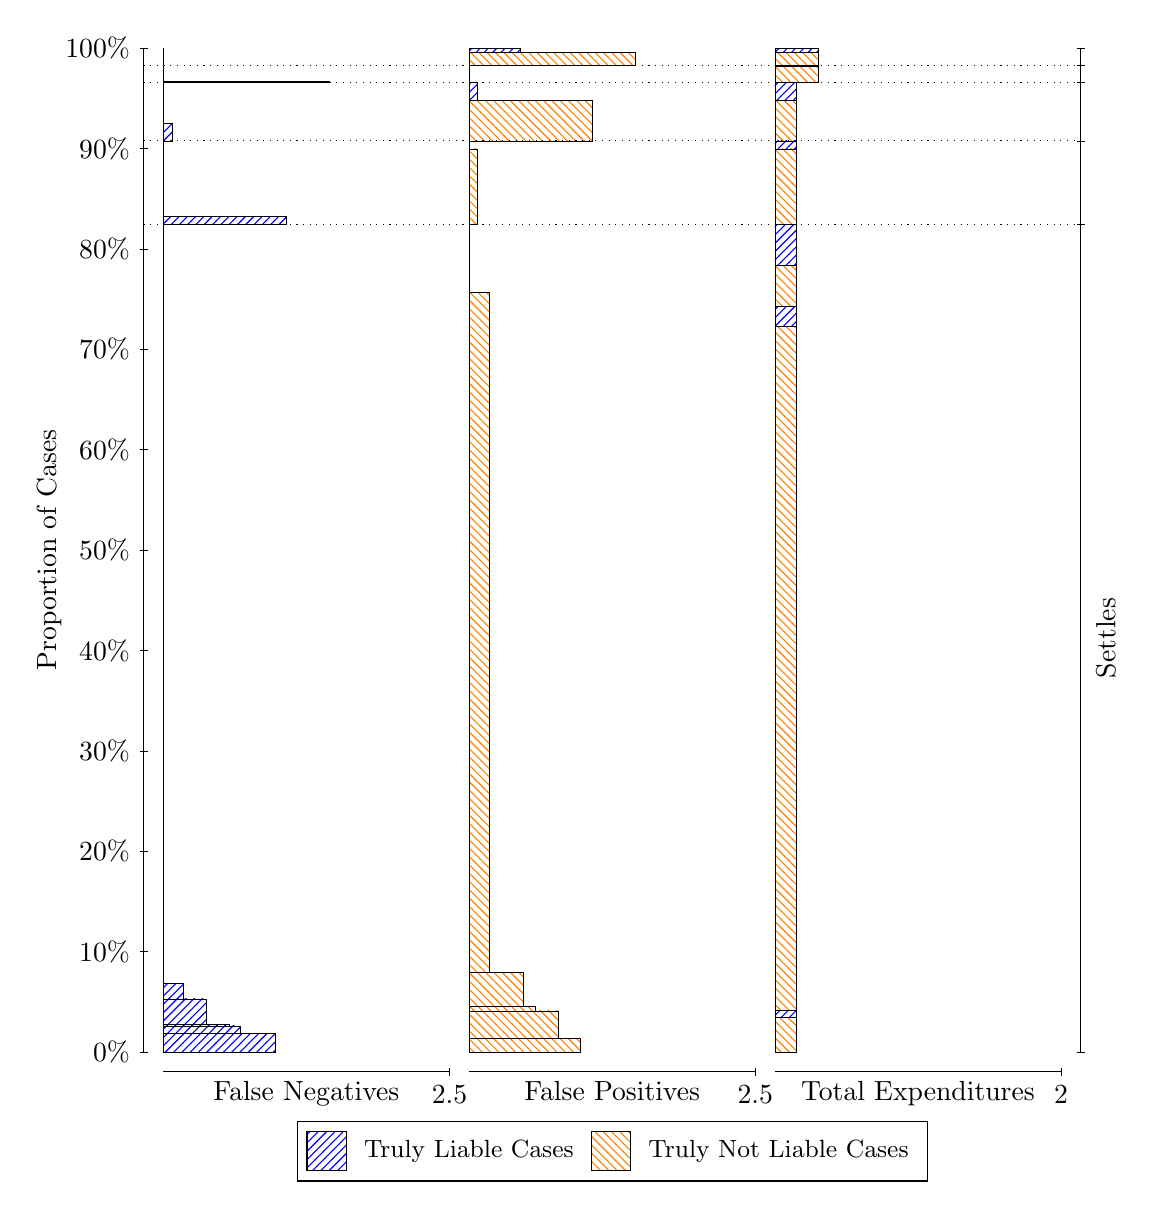
\begin{tikzpicture}
\draw[black, very thin] (1.5,1.75) -- (1.5,14.5);
\node[rotate=90, text=black, anchor=center] at (0.3, 8.125) {Proportion of Cases};
\draw[black, very thin] (1.45,1.75) -- (1.55,1.75);
\node[text=black, anchor=east] at (1.45, 1.75) {0\%};
\draw[black, very thin] (1.45,3.025) -- (1.55,3.025);
\node[text=black, anchor=east] at (1.45, 3.025) {10\%};
\draw[black, very thin] (1.45,4.3) -- (1.55,4.3);
\node[text=black, anchor=east] at (1.45, 4.3) {20\%};
\draw[black, very thin] (1.45,5.575) -- (1.55,5.575);
\node[text=black, anchor=east] at (1.45, 5.575) {30\%};
\draw[black, very thin] (1.45,6.85) -- (1.55,6.85);
\node[text=black, anchor=east] at (1.45, 6.85) {40\%};
\draw[black, very thin] (1.45,8.125) -- (1.55,8.125);
\node[text=black, anchor=east] at (1.45, 8.125) {50\%};
\draw[black, very thin] (1.45,9.4) -- (1.55,9.4);
\node[text=black, anchor=east] at (1.45, 9.4) {60\%};
\draw[black, very thin] (1.45,10.675) -- (1.55,10.675);
\node[text=black, anchor=east] at (1.45, 10.675) {70\%};
\draw[black, very thin] (1.45,11.95) -- (1.55,11.95);
\node[text=black, anchor=east] at (1.45, 11.95) {80\%};
\draw[black, very thin] (1.45,13.225) -- (1.55,13.225);
\node[text=black, anchor=east] at (1.45, 13.225) {90\%};
\draw[black, very thin] (1.45,14.5) -- (1.55,14.5);
\node[text=black, anchor=east] at (1.45, 14.5) {100\%};

\draw[black, very thin] (13.4,1.75) -- (13.4,14.5);
\draw[black, very thin] (13.35,1.75) -- (13.45,1.75);
\node[anchor=west] at (13.35, 1.75) {};
\draw[black, very thin] (13.35,12.263) -- (13.45,12.263);
\node[anchor=west] at (13.35, 12.263) {};
\draw[black, very thin] (13.35,13.32) -- (13.45,13.32);
\node[anchor=west] at (13.35, 13.32) {};
\draw[black, very thin] (13.35,14.062) -- (13.45,14.062);
\node[anchor=west] at (13.35, 14.062) {};
\draw[black, very thin] (13.35,14.279) -- (13.45,14.279);
\node[anchor=west] at (13.35, 14.279) {};
\draw[black, very thin] (13.35,14.5) -- (13.45,14.5);
\node[anchor=west] at (13.35, 14.5) {};

\draw[black, very thin, pattern color=blue, pattern=north east lines] (1.75,1.75) rectangle (3.167,1.986);
\draw[black, very thin, pattern color=blue, pattern=north east lines] (1.75,1.986) rectangle (2.731,2.0802);
\draw[black, very thin, pattern color=blue, pattern=north east lines] (1.75,2.0802) rectangle (2.5857,2.0972);
\draw[black, very thin, pattern color=blue, pattern=north east lines] (1.75,2.0972) rectangle (2.295,2.4236);
\draw[black, very thin, pattern color=blue, pattern=north east lines] (1.75,2.4236) rectangle (2.0043,2.6188);
\draw[black, very thin, pattern color=orange, pattern=north west lines] (1.75,2.6188) rectangle (1.75,12.263);
\draw[black, very thin, pattern color=blue, pattern=north east lines] (1.75,12.263) rectangle (3.3123,12.364);
\draw[black, very thin, pattern color=orange, pattern=north west lines] (1.75,12.364) rectangle (1.75,13.32);
\draw[black, very thin, pattern color=blue, pattern=north east lines] (1.75,13.32) rectangle (1.859,13.546);
\draw[black, very thin, pattern color=orange, pattern=north west lines] (1.75,13.546) rectangle (1.75,14.062);
\draw[black, very thin, pattern color=blue, pattern=north east lines] (1.75,14.062) rectangle (3.8573,14.08);
\draw[black, very thin, pattern color=orange, pattern=north west lines] (1.75,14.08) rectangle (1.75,14.279);
\draw[black, very thin, pattern color=orange, pattern=north west lines] (1.75,14.279) rectangle (1.75,14.44);
\draw[black, very thin, pattern color=blue, pattern=north east lines] (1.75,14.44) rectangle (1.75,14.5);
\draw[black, very thin, pattern color=orange, pattern=north west lines] (5.6333,1.75) rectangle (7.0503,1.9222);
\draw[black, very thin, pattern color=orange, pattern=north west lines] (5.6333,1.9222) rectangle (6.7597,2.2721);
\draw[black, very thin, pattern color=orange, pattern=north west lines] (5.6333,2.2721) rectangle (6.469,2.3245);
\draw[black, very thin, pattern color=orange, pattern=north west lines] (5.6333,2.3245) rectangle (6.3237,2.7616);
\draw[black, very thin, pattern color=orange, pattern=north west lines] (5.6333,2.7616) rectangle (5.8877,11.394);
\draw[black, very thin, pattern color=blue, pattern=north east lines] (5.6333,11.394) rectangle (5.6333,12.263);
\draw[black, very thin, pattern color=orange, pattern=north west lines] (5.6333,12.263) rectangle (5.7423,13.218);
\draw[black, very thin, pattern color=blue, pattern=north east lines] (5.6333,13.218) rectangle (5.6333,13.32);
\draw[black, very thin, pattern color=orange, pattern=north west lines] (5.6333,13.32) rectangle (7.1957,13.836);
\draw[black, very thin, pattern color=blue, pattern=north east lines] (5.6333,13.836) rectangle (5.7423,14.062);
\draw[black, very thin, pattern color=orange, pattern=north west lines] (5.6333,14.062) rectangle (5.6333,14.262);
\draw[black, very thin, pattern color=blue, pattern=north east lines] (5.6333,14.262) rectangle (5.6333,14.279);
\draw[black, very thin, pattern color=orange, pattern=north west lines] (5.6333,14.279) rectangle (7.7407,14.44);
\draw[black, very thin, pattern color=blue, pattern=north east lines] (5.6333,14.44) rectangle (6.2873,14.5);
\draw[black, very thin, pattern color=orange, pattern=north west lines] (9.5167,1.75) rectangle (9.7892,2.1871);
\draw[black, very thin, pattern color=blue, pattern=north east lines] (9.5167,2.1871) rectangle (9.7892,2.2813);
\draw[black, very thin, pattern color=orange, pattern=north west lines] (9.5167,2.2813) rectangle (9.7892,10.966);
\draw[black, very thin, pattern color=blue, pattern=north east lines] (9.5167,10.966) rectangle (9.7892,11.219);
\draw[black, very thin, pattern color=orange, pattern=north west lines] (9.5167,11.219) rectangle (9.7892,11.741);
\draw[black, very thin, pattern color=blue, pattern=north east lines] (9.5167,11.741) rectangle (9.7892,12.263);
\draw[black, very thin, pattern color=orange, pattern=north west lines] (9.5167,12.263) rectangle (9.7892,13.218);
\draw[black, very thin, pattern color=blue, pattern=north east lines] (9.5167,13.218) rectangle (9.7892,13.32);
\draw[black, very thin, pattern color=orange, pattern=north west lines] (9.5167,13.32) rectangle (9.7892,13.836);
\draw[black, very thin, pattern color=blue, pattern=north east lines] (9.5167,13.836) rectangle (9.7892,14.062);
\draw[black, very thin, pattern color=orange, pattern=north west lines] (9.5167,14.062) rectangle (10.062,14.262);
\draw[black, very thin, pattern color=blue, pattern=north east lines] (9.5167,14.262) rectangle (10.062,14.279);
\draw[black, very thin, pattern color=orange, pattern=north west lines] (9.5167,14.279) rectangle (10.062,14.44);
\draw[black, very thin, pattern color=blue, pattern=north east lines] (9.5167,14.44) rectangle (10.062,14.5);
\draw[black, dotted] (1.5,12.263) -- (13.4,12.263);
\draw[black, dotted] (1.5,13.32) -- (13.4,13.32);
\draw[black, dotted] (1.5,14.062) -- (13.4,14.062);
\draw[black, dotted] (1.5,14.279) -- (13.4,14.279);
\draw[black, very thin] (1.75,1.5) -- (5.3833,1.5);
\node[text=black, anchor=north] at (3.5667, 1.5) {False Negatives};
\draw[black, very thin] (5.3833,1.45) -- (5.3833,1.55);
\node[text=black, anchor=north] at (5.3833, 1.45) {2.5};

\draw[black, very thin] (5.6333,1.5) -- (9.2667,1.5);
\node[text=black, anchor=north] at (7.45, 1.5) {False Positives};
\draw[black, very thin] (9.2667,1.45) -- (9.2667,1.55);
\node[text=black, anchor=north] at (9.2667, 1.45) {2.5};

\draw[black, very thin] (9.5167,1.5) -- (13.15,1.5);
\node[text=black, anchor=north] at (11.333, 1.5) {Total Expenditures};
\draw[black, very thin] (13.15,1.45) -- (13.15,1.55);
\node[text=black, anchor=north] at (13.15, 1.45) {2};

\node[text=black, centered, rotate=90] at (13.72, 7.0063) {Settles};





\draw (7.449999999999999,1.5) node[draw=none] (baseCoordinate) {};
\begin{scope}[align=center]
        \matrix[scale=0.5, draw=black, below=0.5cm of baseCoordinate, nodes={draw}, column sep=0.1cm]{
            \node[rectangle, draw, minimum width=0.5cm, minimum height=0.5cm, pattern color=blue, pattern=north east lines] {}; &
            \node[draw=none, font=\small, text=black] (B) {Truly Liable Cases}; &
            \node[rectangle, draw, minimum width=0.5cm, minimum height=0.5cm, pattern color=orange, pattern=north west lines] {}; &
            \node[draw=none, font=\small, text=black] (B) {Truly Not Liable Cases}; \\
            };
\end{scope}

\end{tikzpicture}
\end{document}